\section{System design}
\label{sec:system_design}
~

No supervised learning model has been designed to 
tackle the non-preemptive, global fixed-priority scheduling problem 
for DAG tasks.
Therefore, we must first design a supervised learning model.

In supervised learning, the machine learning model 
predicts an output (forward pass) and then computes the error between
the predicted output and a known true output.
The gradient of the error function is then propagated through the network to tweak the model's 
trainable parameters, which is also called the backward pass (see Figure \ref{fig:supervised_learning}).

\begin{figure}
    \centering
    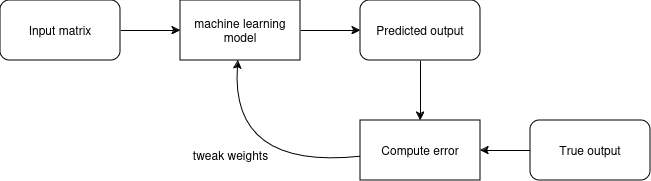
\includegraphics[width=\linewidth]{images/supervised_learning_diagram.drawio.png}
    \caption{The supervised learning method.}
    \label{fig:supervised_learning}
\end{figure}

\subsection{Supervised design}
~

\subsubsection{Input DAGs}
~

Each input DAG  task will be represented using 
a matrix of numbers with each row being a node
and each column being a raw feature of a node.
The list of raw features is similar to what is proposed by \citet{Lee2021GlobalDagSchedDRL},
that is :
\begin{list}{}{}
    \item - the normalized wcet of the node, i.e., $C_i / L$ for node $i$ with $L$ being the total workload ;
    \item - the number of incoming neighbours ;
    \item - the number of outgoing neighbours ;
    \item - a boolean value of whether the node is the source or sink node ;
    \item - a boolean value of whether the node is part of the critical path of the DAG.
\end{list}

The wcet is widely used as a criteria for priority-list scheduling algorithm (RM, EDF\cite{buttazzo2005RMvsEDF}, etc.)
but it needs to be normalized to have the context information of the whole graph.
The number of incoming and outgoing neighbours makes it possible 
to take into account the inner structure of the graph to compute the execution order.
The source and sink nodes are particular nodes in that their priority
is not important because they will respectively execute first and last due to their dependency constraints.
Finally, the critical path plays a huge role in state-of-the-art heuristics\cite{He2019DagIntra}\cite{zhao2020DAGsched},
with nodes in the critical path often having higher priorities than those
that aren't.
An example of such a DAG task representation is shown in Figure \ref{fig:dag_task_matrix_example}.

\begin{figure}
    \centering
    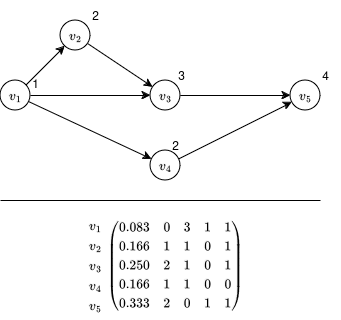
\includegraphics[width=\linewidth]{images/dag_matrix_example.drawio.png}
    \caption{Example dag task with 5 nodes a total workload of 12
    and the matrix representation of each node with the column respectively being the above list of features.}
    \label{fig:dag_task_matrix_example}
\end{figure}

\subsubsection{Output labels}
~

An Integer Linear Programming (ILP) solver will be used to compute
the optimal (minimum makespan) schedule for each DAG task and then
ordering the nodes according to their release time in the ILP schedule.

The output of the model will be a matrix of probabilities,
with each row being the index of a node and each column being the index of the priority.
There are as many priorities as there are nodes and 
the priority list of each DAG is then retrieved using the column
index of the maximum probability as the assigned probability, for each row.
Matrix output example for the DAG task shown in Figure \ref{fig:dag_task_matrix_example}
is shown in Figure \ref{fig:dag_output_matrix_example}.

\begin{figure}
    \centering
    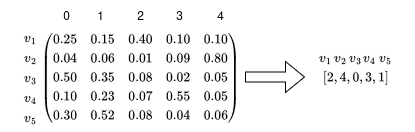
\includegraphics[width=\linewidth]{images/output_matrix_example.drawio.png}
    \caption{Example of an matrix output from the model, the predicted list of priorities (on the right)
    is retrieved from the probabilities.}
    \label{fig:dag_output_matrix_example}
\end{figure}

The ILP output matrix to compare the predicted output to is of the same shape
as the predicted output matrix with the probabilities being 1 on the optimal priority for each row 
, and 0 otherwise.

\subsubsection{Loss function}
~

The problem is being treated as a classification problem,
hence the binary cross-entropy loss function will be used.
This function is defined as follows :
\begin{equation}
    loss(x, y) = \sum_{i=1}^{n} -y_i\log(x_i)
\end{equation}
    
where $x$ is the flattened matrix representing the predicted output,
$y$ is the flattened matrix representing the true output (ILP output),
and $n$ is the number of element in $x$ and $y$.


\subsection{Model design}
~

The model's architecture is very similar to the proposed encoder in \citet{Lee2021GlobalDagSchedDRL},
that is, the model is comprised of three modules.
Two feed forward networks and one attention-based graph convolutional network (see Figure \ref{fig:model_diagram}).

\begin{figure}
    \centering
    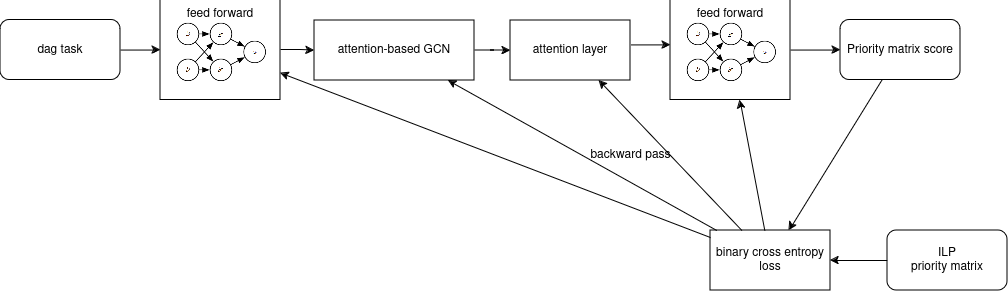
\includegraphics[width=\linewidth]{images/designed_model.png}
    \caption{The architecture diagram of the proposed supervised machine learning model.}
    \label{fig:model_diagram}
\end{figure}

\subsubsection{Feed forward networks}
~

The two feed forward networks have 3 layers with each 
layer $n$ producing the following output,
where $W_n \in \mathbb{R}^{5\times5}$ is the matrix of trainable weights
at layer $n$, $b_n \in \mathbb{R}^5$ is the bias and $X_n$ is either a node's vector representation
or the output of the previous layer, and $ReLU(x) = max(0, x)$:
\begin{equation}
    o_{n} = ReLU(W_{n}X_{n} + b_n),\, n \in \{1,2,3\}
\end{equation}
There is an exception for the second feed forward network where the last 
layer's output is computed using the following equation:
\begin{equation}
    o_{3} = \tanh(W_{3}X_{3} + b_3)
\end{equation}
where $W_3 \in \mathbb{R}^{nbPriorities \times 5}$,
$b_3 \in \mathbb{R}^{nbPriorities}$ and $\tanh$ is the 
hyperbolic tangent activation function.
Also, $nbPriorities$ corresponds to the number of different priorities
that can be assigned to each node.


\subsubsection{Graph Convolutional Network}
~


For each gcn layer, the input vector $X_k$ 
goes through an aggregation phase where,
given the set of incoming neighbours of node $v_i$, $\mathcal{N}_{in}(v_i)$, which includes
$v_i$, and the set of outgoing neighbours $\mathcal{N}_{out}(v_i)$, which also includes $v_i$,
the next vector representation $X_{k+1}$ is calculated by the following equations:

$$
\begin{array}{l}
AttentionModule(X_i) = \sum_{j \in \mathcal{N}(v_i)} \alpha_{ij} X_j
\end{array}
$$

\begin{figure}
    \centering
    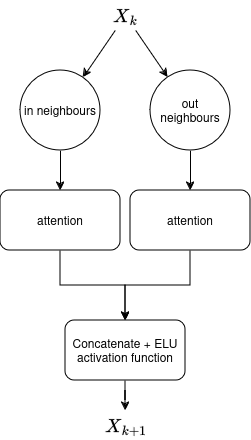
\includegraphics[width=0.5\linewidth]{images/gcn_update_aggregate_diagram.png}
    \caption{Diagram of the graph convolution network layer. $X_k$ is the transformed node vector representation
    and ELU is the exponential linear unit function (see Equation \ref{eq:elu}).}
    \label{fig:update_aggregate_diagram}
\end{figure}

\begin{equation}
\text{ELU}(x) = 
\begin{cases}
x, & \text{if } x > 0 \\
\exp(x) - 1, & \text{if } x \leq 0
\end{cases}
\label{eq:elu}
\end{equation}


% config for 20,30 nodes : 
%  "dag_config": {
%    "parallelism": 8,
%    "layer_num_min": 5,
%    "layer_num_max": 8,
% config for 10 nodes :
%"dag_config": {
%    "parallelism": 8,
%    "layer_num_min": 3,
%    "layer_num_max": 8,
% config for 40 nodes :
%"dag_config": {
%    "parallelism": 8,
%    "layer_num_min": 7,
%    "layer_num_max": 10,
% config for 50 nodes :
%"dag_config": {
%    "parallelism": 8,
%    "layer_num_min": 10,
%    "layer_num_max": 15,
%config for varying number of parallelism (n=30nodes)
%"dag_config": {
%    "parallelism": [4-6, 7],
%    "layer_num_min": 8, (5 for p = 7)
%    "layer_num_max": 13, (10 for p = 7)